\graphicspath{{./ch_LDE_teleportation_SI/figures/}}

\chapter{Teleportation}

\section{Conventions}

The basis states used for the electrons are $\ket{0} = \ket{\mszero}$ and $\ket{1} = \ket{\msmone}$. For the nitrogen, $\ket{0} = \ket{\mizero}$ and $\ket{1} = \ket{\mimone}$. When specifying joint quantum states, the first qubit is the nitrogen on site A, the second the electron on site A, and the third the electron on site B. Teleportation is performed from qubit 1 onto qubit 3.

By $x, y, z$ we denote $\pi/2$ rotations around the $+X, +Y, +Z$ axes respectively. Bars over gate symbols indicate negative rotation sense. In the measurement sequences, rotations around $+X, +Y$ correspond to phases of the applied driving pulses of $+90^\circ$ and $0^\circ$, respectively. We prepare $\ket{x} \equiv (\ket{0}+\ket{1})/\sqrt2$ by $y \ket{0}$ and $\ket{y} \equiv (\ket{0}+\mathrm i \ket{1})/\sqrt2 = \bar{x}\ket{0}$. Capital letters $X, Y, Z$ indicate $\pi$ rotations.

\subsubsection{Hamiltonian of Alice}

The relevant energy levels of the electron and nuclear spins of Alice are depicted in Fig.~\ref{fig:teleportation-SOM_system-Alice}a. We chose the rotating frame (Fig.~\ref{fig:teleportation-SOM_system-Alice}b) such that the relevant Hamiltonian without driving can be written as
\be
    \mathcal{H}^\mathrm A_0 = 
    \begin{pmatrix}
        -A & 0 & 0 & 0 \\
        0 & 0 & 0 & 0 \\
        0 & 0 & 0 & 0 \\
        0 & 0 & 0 & 0
    \end{pmatrix},
\ee
where $A = 2\pi \times 2.19$\,MHz is the parallel hyperfine coupling constant of electron and nitrogen at low temperatures. The spin eigenstates are $\ket{00}, \ket{01}, \ket{10}, \ket{01}$.

\section{Desired state evolution}

\subsection{Source state preparation}

After generating entanglement, we start with the state 
\be
    \ket{1} \left ( \ket{01} - \ket{10} \right ) / \sqrt{2}. 
\ee
We perform the desired rotation on the nitrogen spin for the $\msmone$ manifold, then apply a $\pi$-pulse to the electron and repeat the operation. In this way the operation on the nitrogen spin is unconditional on the electron state and the electron phase is protected by a spin-echo. With an RF operation $\ket1 \mapsto \alpha\ket0 + \beta\ket1$ this procedure yields
\begin{widetext}
\be
    \frac{1}{\sqrt 2} \left( 
        \left(\expe^{-\ii A(t-t_0)} \alpha \ket0 + 
            \beta \ket1 \right) \ket{00}
        + \left( \alpha \ket0 + \beta \ket1 \right) \ket{11}
    \right).
\ee
\end{widetext}
Note that the states associated with $\ket{00}$ on Alice's side accumulate a phase during free evolution time, $t$, due to the choice of rotating frame. $t_0$ is the time at which the $\pi$-pulse on the electron is performed during preparation. By chosing the evolution time such that $A(t-t_0)$ is a multiple of $2\pi$ the initial state can be factorized. We implement the unconditional rotation of the electron spin with a CORPSE pulse that provides a $\pi$ rotation that is insensitive against detuning over a range of a few MHz\cite{2003PhRvA..67d2308C}.


\subsection{Bell-state measurement}

The BSM consists of a CNOT rotation around the $+Y$ axis on Alice's electron spin, conditional on the nitrogen spin being in $\ket0$, followed by a $\pi/2$ rotation around the $+Y$ axis on the nitrogen spin. We implement the CNOT by rotating $\mimone$ by $\pi$ and $\mizero$ by $2\pi$, achieved by a pulse with Rabi frequency $A/\sqrt{3}$. During this pulse Alice's states $\ket{00}$ and $\ket{01}$ are not unaffected. In particular, the time-dependent phase of the state $\ket{00}$ is reduced compared to not performing the pulse (or compared to the case of an ideal CNOT gate in which only a real $\mathbb{1}$ operation would be applied to this state) because some population temporarily leaves this state. Conversely, $\ket{01}$ will acquire some phase because some population will temporarily be in $\ket{00}$. An unconditonal rotation of the nitrogen spin is achieved in the same was as for preparation, by performing the operation twice, with an electron flip in between. After these gate operations we have
\begin{align}
    \frac{1}{2} \bigg[
          & \ket{00} \left( \beta\ket0 - 
            \expe^{\ii\lambda}\alpha\ket1 \right) \notag\\
        + & \ket{01} \left( \expe^{-\ii A(t_1-t_0)-\ii\kappa}\alpha\ket0 +
            \beta\ket1 \right) \notag\\
        + & \ket{10} \left( -\beta\ket0 - 
            \expe^{\ii\lambda}\alpha\ket1 \right) \notag\\
        + & \ket{11} \left( \expe^{-\ii A(t_1-t_0)-\ii\kappa}\alpha\ket0 -
            \beta\ket1 \right)
    \bigg],
\end{align}
where $t_1$ is the time of the $\pi$-pulse on the electron and $\lambda,\kappa$ are the additional phases on $\ket{00}$ and $\ket{01}$.

\subsection{Phase calibration}

We can eliminate the undesired phases before the teleportation experiment by calibrating the rotation axis of the $\pi/2$ operation on the nitrogen in the BSM and the evolution times. After initializing the nitrogen and electron spin states of Alice into $\ket{1}(\ket{0} - \ket{1})/\sqrt{2}$ (equivalent to the entanglement operation on Alice, ignoring Bob), we prepare the nitrogen in $\ket{\bar x} = (\ket{0} - \ket{1})/\sqrt{2}$ (preparation operation is $y$) and perform the BSM, yielding
\begin{align}
    \frac{1}{2\sqrt2} \bigg[
          & \ket{00} \left( -1 - \expe^{\ii\lambda} \right) \notag\\
        + & \ket{01} \left( -1 + 
            \expe^{-\ii A(t_1-t_0) -\ii\kappa} \right) \notag\\
        + & \ket{10} \left( 1 - \expe^{\ii\lambda} \right) \notag\\
        + & \ket{11} \left( 1 + \expe^{-\ii A(t_1-t_0) -\ii\kappa} \right)
    \bigg]
\end{align}
before readout (Fig.~\ref{fig:teleportation-SOM_BSM-calibration}). We sweep the rotation axis of the RF pulse on the nitrogen (affecting the phase $\ii\lambda$) and subsequently the evolution time between the CNOT and $Y$ operations during the BSM (affecting the phase $-\ii A(t_1-t_0) -\ii\kappa$). Calibration is achieved by maximizing the probabilities for outcomes $\ket{00}$ and $\ket{11}$. 

\paragraph{Dynamical decoupling of Bob's electron spin}

To protect the target state against dephasing during the BSM, we perform an XY4 decoupling sequence in parallel. The first $\pi$-pulse of this echo sequence is the $\pi$-pulse performed during the entanglement generation attempt. The remaining X-Y-X sequence is executed during the BSM. Taking these additional rotations into account, the total state before readout, including phase calibration, is
\begin{align}
    \label{eq:BSM-outcomes}
    \frac{1}{2} \bigg[
          & \ket{00} \left( \alpha\ket0 + \beta\ket1 \right) \notag\\
        + & \ket{01} \left( -\beta\ket0 + \alpha\ket1 \right) \notag\\
        + & \ket{10} \left( \alpha\ket0 - \beta\ket1 \right) \notag\\
        + & \ket{11} \left( \beta\ket0 + \alpha\ket1 \right)
    \bigg].
\end{align}
Because we do not intialize the nuclear spin on Bob's side we perform all electron spin rotations with CORPSE pulses\cite{2003PhRvA..67d2308C}.

\subsubsection{Feed-forward}
The required feed-forward operations to re-create $\ket{\psi}$ on the target spin can be taken straight-forward from Eq.~\ref{eq:BSM-outcomes}. For the estimation of the fidelity of the teleported state with the ideal source state it is sufficient to read out in the basis aligned with the source state vector. We achieve this readout by modifying the feed-forward operation such that we rotate the target state $U_{i,j}\ket \psi$ directly into the $z$-basis, conditional on the outcome of the BSM. The operations we apply in practice are summarized in Table \ref{tab:psiminus-operations}.

\section{Data analysis}

For each input state we determine the number of events $n_{0}$ and $n_{1}$ that give measurement outcomes $\mszero$ and $\msmone$, respectively. The probability amplitudes $c_0$ and $c_{1}$ for $\ket0$ and $\ket1$ are obtained by performing readout correction using the readout fidelities $F_0$ and $F_{-1}$ for $\mszero$ and $\msmone$, respectively. We obtain $F_0$ and $F_{-1}$ from calibration measurements performed periodically during the experiment. The teleportation fidelity of the state is given by either $c_0$ or $c_{1}$ (see Table~\ref{tab:psiminus-operations}).

The uncertainty of $c_0$ and $c_1$ is determined by the standard deviation of the binomial distribution with probabilities $n_0/(n_0 + n_1)$ and $n_1/(n_0 + n_1) = 1 - n_0/(n_0 + n_1)$, and the measurement uncertainties of $F_0$ and $F_{-1}$ (for both readout fidelities the measurement uncertainties are $\lesssim 0.005$).

\section{Error model}

In the following we describe the errors we take into account for modeling our experimental results. Any further errors are considered small in comparison and we ignore them in this discussion. In particular we assume that the preparation of the source state $\ket\psi$ is not subject to errors resulting from RF or microwave pulses.

Note that we model the experimental results numerically with the best guesses of the empiric parameters described below, without treatment of their uncertainties.

In general we simulate the experimental results by modeling the system by a $2\times 2 \times 2$ dimensional density matrix that is subjected to operators that correspond to the operations physically applied. Treatment of errors is included in the description of the types of errors taken into consideration in the following. Operations for which no error is listed are assumed to be perfect.

\subsection{CNOT pulses}

The fidelity of Alice's electron spin rotations that are selective on the \nfourteen\ spin state are limited by the finite linewidth of the electron spin transitions. We simulate the effect of the pulse on the different hyperfine populations by evaluating the probability for inversion versus detuning using a master equation solver \cite{2013CoPhC.184.1234J}, 
and integrating over the transition line shapes. In this way we compute the probabilities for an erroneous inversion for $m_\mathrm I = -1$ and non-inversion for $m_\mathrm I = 0$ to be both 0.01. Our calculation is based on a finite linewidth that is determined by the electron spin dephasing time, $T_2^* = 2\,\mu\mathrm s$. In our model we assume that in case of an error the spin state is dephased (i.e., we numerically set the respective coherences in the resulting density matrix to zero).

\subsection{Nuclear spin initialization}

When preparing the source state to be teleported, the following errors can occur: (1) Initialization by measurement into $\mimone$ succeeds with a fidelity $p_{-1}$, and fails for the initial state in either $\mizero$ or $\mipone$, with probabilities $p_0$ and $p_{+1}$, respectively; (2) After each failed attempt to generate entanglement between Alice and Bob the electron is reset by optical spin-pumping\cite{2013Natur.497...86B}. 
During this reset to $\mszero$ the nuclear spin can flip --- with $\Delta m_\mathrm I = \pm 1$ --- with a probability $p_\text{flip}$\cite{2010Sci...329..542N}.

Assuming that the conditional probability for a nuclear spin flop accompanying an electron spin flip, $p_\text{flip}$, is identical for all $\Delta m_\mathrm I = \pm 1$, the equations describing the changes of populations in dependence of the number of electron spin flips, $n$, are
\begin{widetext}
\begin{align}
   \label{eq:teleportation-SOM_Nspinpopulations}
   p_{-1}(n) - p_{-1}(n-1) &= p_\text{flip} 
       \left( p_{0}(n-1) - p_{-1}(n-1) \right) \notag\\
   p_{0}(n) - p_{0}(n-1) &= p_\text{flip}
       \left( -2 p_{0}(n-1) + p_{-1}(n-1) + p_{+1}(n-1) \right) \notag \\
   p_{+1}(n) - p_{+1}(n-1) &= p_\text{flip}
       \left( p_0(n-1) - p_{+1} (n-1) \right).
\end{align}
\end{widetext}
The measured population of $\mimone$ in dependence of $n$ is shown in Fig.~\ref{fig:teleportation-SOM_Nspinflips}.

From independent calibration measurements we estimate the nuclear spin to be initialized by measurement with $p_{-1}(0) = 0.97$, $p_{0}(0) = 0.02$, and $p_{+1}(0) = 0.01$. Together with the nuclear spin depolarization during subsequent entanglement generation attempts we determine $\langle p_{-1} \rangle = 0.88$, $\langle p_{0} \rangle = 0.10$, and $\langle p_{+1} \rangle = 0.02$ from the solution of (\ref{eq:teleportation-SOM_Nspinpopulations}), for a maximum of 250 entanglement generation attempts before re-initialization by measurement. Here,
\be
    \langle p_{i} \rangle = \frac{1}{N} \sum_{n=0}^{N} p_{i}(n)
\ee
is the average population of the nuclear spin state $i$ for a maximum of 2N entanglement generation attempts. Note that the electron spin is in a superposition before reset, and thus the number of spin flips is half the number of entanglement generation attempts. The probability for successful entanglement generation is independent of the attempt number.

In the simulation of the experimental data we calculate the projected outcomes for each of the nuclear spin states and determine the combined result by weighing the average with $\langle p_{-1} \rangle$, $\langle p_{0} \rangle$, and $\langle p_{+1} \rangle$. Because population in $\mipone$ is outside the simulated space of two-level systems we treat this case in a separate simulation before weighing. The net effect of detuned MW pulses in this case is determined by calculating the electron spin rotation versus detuning and integrating over the $\mipone$ transition line shape.

The influence of imperfect nuclear spin initialization can also be approximated inituitively as follows: for $\mipone$ none of the operations on Alice's side are performed since all pulses applied are off-resonant, leading to dephasing of the state and ultimately a fully random outcome of Bob's readout. Initialization in $\mizero \equiv \ket0$ results in the opposite outcome than the one obtained from correct intialization in $\mimone \equiv \ket1$. Thus, with probability $2 \langle p_{0} \rangle + \langle p_{+1} \rangle$ the target state is fully mixed.

\subsection{Readout}
\label{sec:readout-error}

The major limitation of the Bell-state measurement fidelity is the finite single-shot readout fidelity of both electron and nuclear spin on Alice's side. Electron spin readout is achieved by resonant optical excitation of $E_y$. Detection of a least one photon during this interval is registered as readout result $\mszero$, otherwise the result is $\mspmone$. Nuclear spin readout is achieved by re-setting the electron spin to $\mszero$, mapping the nuclear spin state onto the electron spin by a CNOT, and reading out the electron spin. This procedure is performed twice in order to maximize the readout fidelity\cite{Robledo:2011fs}. 
Readout result $\mizero$ is obtained for detection of at least one photon during either round.

The electron spin readout is limited by finite photon collection efficiency and electron spin mixing in the excited state\cite{Robledo:2011fs}. 
For Alice, we measure a mean single-shot readout fidelity of $F_\text{e-RO} = 0.963 \pm 0.005$. The nuclear spin readout is additionally limited by the CNOT fidelity. With two readout rounds we estimate a mean readout fidelity of $F_\text{N-RO} = 0.985$ from the electron spin readout and CNOT pulse simulations.

In the simulation of the experimental results we use the single-shot readout fidelities to determine the conditional density matrices that arise after measuring the electronic and nuclear spin.

\subsection{Photon indistinguishability and entangled state fidelity}
\label{sec:lde-visibility}

The entangled state between the two electronic spins can be modeled as
\be
    \rho = V | \Psi^- \rangle \langle \Psi^- | + \frac{(1-V)}{2} \left( \ket{01}\bra{01} + \ket{10}\bra{10} \right ),
\ee
where the visibility $V$ describes the distinguishability between the photons emitted from Alice and Bob. Here we assume that all other imperfections are negligible compared to the photon distinguishability. The limitations of the Bell state fidelity are discussed in detail in Bernien {\em et al.}\cite{2013Natur.497...86B}

For modelling we treat $V$ as a free parameter used to match the average teleportation fidelity. Using the parameters as described above and setting $V = 0.74$ (corresponding to a Bell-state fidelity of $F_{\Psi^-}$ = 0.87) our simulation yields a mean teleportation fidelity of $F = 0.77$.

\section{Further analysis of the teleporter performance}

\subsection{Effect of the feed-forward operation}

Figure~4B of the main text shows the teleportation fidelity when no feed-forward is performed. This data is extracted from the teleportation data including feed-forward in the following way. We first determine the probability for obtaining the expected readout result independently for each BSM outcome by postselection. We then invert the readout result for all operations with a negative rotation sense. In this way we obtain the result that would have been measured if for each BSM outcome the same qubit rotation was performed (i.e., no feed-forward). We assume that any experimental errors in the final readout pulse are small and thus neglect them in this treatment.

\subsection{Correction for intialization}

After determining the entangled state fidelity as described above we can estimate the actual teleportation fidelity by assuming perfect intialization in our simulation. Setting $p_{-1} = 1$ we compute a mean teleportation fidelity of $F_\text{corrected} = 0.86$ (Fig.~\ref{fig:more_fidelities}A).

\subsection{Teleportation fidelity by Bell-state measurement outcome}

Due to the different readout fidelities for each of the four Bell states (see above and Fig.~3 in the main text) we can expect different teleportation fidelities as well. We find that the teleportation fidelity by outcome of the Bell-state measurement is consistent with expectations (Fig.~\ref{fig:more_fidelities}B), but the statistical uncertainty prevents a more detailed discussion.

\subsection{Probability of BSM outcomes}


We verify in more detail that the teleportation works as intended by examining the distribution of BSM outcomes obtained from all teleportation events (Fig.~\ref{fig:more_fidelities}C). The simulations are in good agreement with the data. The deviation from an equal probability of 0.25 for all BSM outcomes is mainly due to the asymmetry in the readout fidelities of the electron spin states\cite{Robledo:2011fs}.

\clearpage

\begin{figure*}[p]
    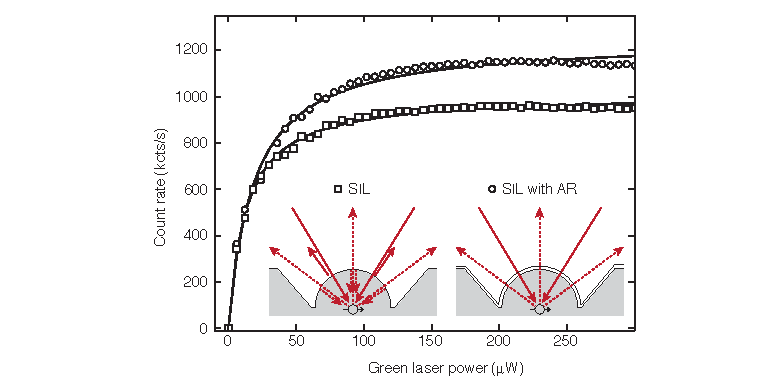
\includegraphics{AR_coating}
    \caption{
    \label{fig:AR-SIL}
    Saturation measurements on SILs with and without antireflection coating. 
    Fluorescence count rates in dependence of off-resonant green excitation power (kcts = 1000 counts). Solid lines are fits to $A \cdot x / (x + P_\text{sat})$. In the case of a bare SIL, photons emitted from the NV centre and the excitation laser can be reflected at the interface due to the large refractive index of diamond. This effect is overcome by an antireflection coating which further increases the count rates and significantly reduces reflections of the excitation laser.
    }
\end{figure*}

\clearpage

\begin{figure*}[p]
    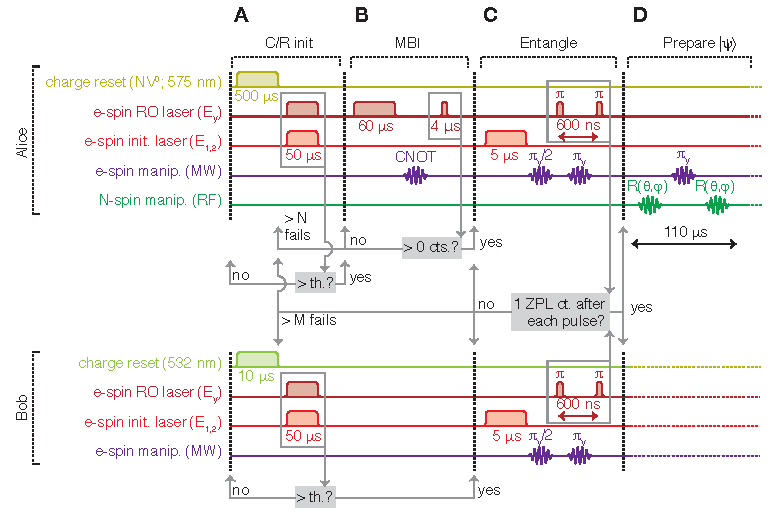
\includegraphics{conditional_init}
    \caption{
    \label{fig:teleportation-init} 
    System initialization.
    \textbf{A,} We verify charge and resonance condition of Alice and Bob (asynchronously) by applying laser pulses on $E_y$ and $E_{1,2}$ simultaneously and putting a lower threshold on the number of phonon side band photons detected during those pulses. If the threshold is not met we reset the charge state: On Alice, we repump NV$^0$ $\rightarrow$ NV$^-$ using a laser at 575\,nm, on resonance with the ZPL of NV$^0$\cite{Siyushev:2013en}. 
    On Bob, we use off-resonant excitation at 532\,nm. We repeat verification and repump until success.
    \textbf{B,} Following spin-pumping into $\mspmone$ by excitation of $E_y$ we apply a CNOT on the electronic spin, such that rotation to $\mszero$ is only performed for $\mimone$. A PSB photon detected during a short readout pulse on $E_y$ signals a high-fidelity measurement of $\mszero$ and projection of the nuclear spin into $\mimone$. If no photon is detected, we re-try for a maximum of $N$ times (here, $N=100$), before charge and resonance are re-evalutated. In between attempts we apply $50\,\mu\mathrm s$ of illumination on both $E_y$ and $E_{1,2}$ in order to randomise the nuclear spin owed to off-diagonal terms in the hyperfine interaction in the optical excited state (not shown in the diagram).
    \textbf{C,} As soon as both Alice and Bob are initialised, we attempt to generate entanglement between them. Each attempt starts with an electron spin reset to $\mszero$. Two rounds of optical excitation with optical $\pi$-pulses on $E_y$ follow, separated by a MW $\pi$-pulse. Detection of exactly one ZPL photon after each pulse heralds creation of entanglement. We perform a maximum of $M$ attempts before re-initialisation (here, $M=250$). 
    \textbf{D,} When entanglement is created, we prepare the \nfourteen\ spin of Alice unconditional on the electron spin state, while preserving the electron spin phase. The RF pulse that generates the rotation is only resonant for $\msmone$; we perform the rotation twice, separated by a $\pi$-pulse on the electron.
    }
\end{figure*}

\clearpage

\begin{figure*}[p]
    \centering
    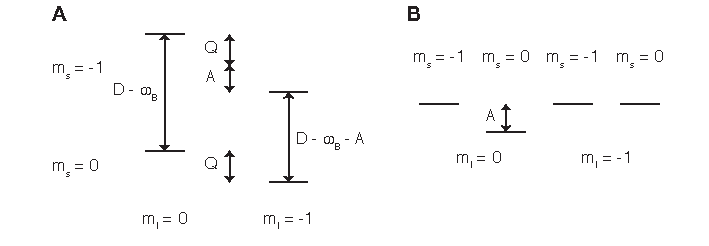
\includegraphics{figure_SOM_system-Alice}
    \caption{
    \label{fig:teleportation-SOM_system-Alice}
    Relevant spin states on Alice's side.
    \textbf{A,} Lab frame. 
    \textbf{B,} Rotating frame chosen. $D = 2\pi \times 2.878\,\text{GHz}$ is the NV electron zero-field splitting, $\omega_\mathrm B \approx 2\pi \times 50$ MHz is the Zeeman splitting of the electron, $A = 2\pi \times 2.19$ MHz is the electron-nitrogen hyperfine coupling constant.}
\end{figure*}

\clearpage

\begin{figure*}[p]
    \centering
    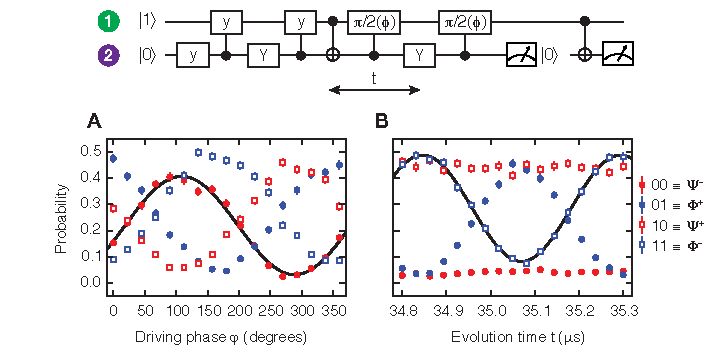
\includegraphics{figure_SOM_BSMcalibration}
    \caption{
    \label{fig:teleportation-SOM_BSM-calibration}
    Calibration of the Bell-state measurement.
    \textbf{A,} Calibration of the driving phase of the Hadamard operation, and 
    \textbf{B,} subsequent calibration of the evolution time between the CNOT gate of the BSM and the electron $\pi$-pulse for the unconditional rotation of the nuclear spin. The solid lines are sinosoidal fits to the BSM outcomes to be maximised. The legend indicates the correspondence between two-qubit measurement results $ij$ and Bell-state detection. The calibration is performed with the full teleportation protocol including the MW pulses during entanglement generation attempts (but without optical $\pi$-pulses). Error bars are 1 s.d.}
\end{figure*}

\clearpage

\begin{figure*}[p]
    \centering
    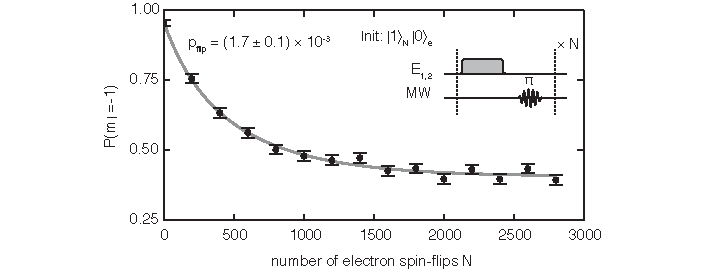
\includegraphics[scale=1]{figure_SOM_Nspinflips}
    \caption{
    \label{fig:teleportation-SOM_Nspinflips}
    Nuclear spin state depolarization as function of electron spin flips by optical spin-pumping.
    We measure nuclear spin flips that are conditional on electron spin flips when optically pumping on $E_{1,2}$. We prepare the nuclear spin in $\msmone$ and measure the probability for its preservation dependent on the number of cycles of electron spin-pumping $\ket 1 \rightarrow \ket 0$ and re-preparation of $\ket 1$ by a microwave $\pi$-pulse. The solid line is a fit to the solution of (\ref{eq:teleportation-SOM_Nspinpopulations}) that is given by $p_{-1}(n) = 1/6 \left( 2 + (1-3p_\text{flip})^N + 3(1-p_\text{flip})^N \right)$ (neglecting initial population in $\mizero$ and $\mipone$). Because the data shown here is not corrected for finite initialisation fidelity of the nuclear spin and nuclear spin readout errors we include an offset $o$ and scaling factor $A$ in the fit function, $p_{-1}(n) = A/6 \left( 2 + (1-3p_\text{flip})^N + 3(1-p_\text{flip})^N \right) + o$. The fit yields a nuclear spin-flip probability of $p_\text{flip} = (0.17\pm0.01)\,\%$ per spin pumping cycle, and $A = 0.83 \pm 0.02$, $o = 0.13 \pm 0.01$. Note that the data shown in Fig.~2D of the main text has been corrected for nuclear spin readout errors. Error bars are 1 s.d.}
\end{figure*}

\clearpage

\begin{figure*}[p]
    \centering
    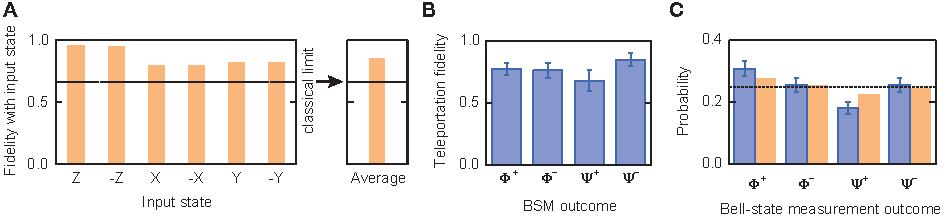
\includegraphics[width=120mm]{more_fidelities}
    \caption{
    \label{fig:more_fidelities}
    Further analysis of the teleportation fidelity.
    \textbf{A,} Correction for imperfect initialization of the source qubit. We simulate the teleportation outcomes using perfect intialization, $p_{-1} = 1$. The simulation yields and average fidelity of 0.86.
    \textbf{B,} We determine the average teleportation fidelity for each outcome of the Bell-state measurement. Within the statistical uncertainty the fidelities do not differ substantially.
    \textbf{C,} Probability for each BSM outcome, as measured (blue) and predicted from the model (orange). The dashed line marks 0.25. Error bars are 1 s.d.
    }
\end{figure*}

\clearpage

\begin{table}[htp]
    \centering
    \caption{
    \label{tab:psiminus-operations}
    Feed-forward and readout operations applied for each BSM outcome.}
    \vspace{.2cm}
    \begin{tabular}{l | c c c c || l}
        Input & $\ket{00}$ & $\ket{01}$ & $\ket{10}$ & $\ket{11}$ & ideal result \\
        \hline
        $\ket{+z} = Y\ket{1}$ & $\mathbb 1$ & $Y$ & $\mathbb 1$ & $Y$ & $\ket{0}$ \\
        $\ket{-z} = \mathbb 1 \ket{1}$ & $Y$ & $\mathbb 1$ & $Y$ & $\mathbb 1$ & $\ket{0}$ \\
        $\ket{+x} = \bar y \ket{1}$ & $\bar y$ & $y$ & $y$ & $\bar y$ & $\ket{0}$ \\
        $\ket{-x} = y \ket{1}$ & $y$ & $\bar y$ & $\bar y$ & $y$ & $\ket{0}$ \\
        $\ket{+y} = \bar x \ket{1}$ & $\bar x$ & $\bar x$ & $x$ & $x$ & $\ket{1}$\\
        $\ket{-y} = x \ket{1}$ & $x$ & $x$ & $\bar x$ & $\bar x$ & $\ket{1}$\\
    \end{tabular}
\end{table}

\clearpage
\bibliographystyle{../thesis}
\bibliography{ch_LDE_teleportation_appendix}


